\section{My contribution}

\subsection{Introduction}

After outlining the context of the work-study program and describing the technique I worked
on, it is finally time to discuss my contributions to the project. First, I will explore 
the design I implemented and explain why this specific design was chosen. Next, we will 
examine the simulation models I developed and their applications. Following this, I will 
detail the optimization and parallelization of the code that was done to enhance its performance. 
Finally, we will discuss how this optimized code could be utilised to estimate uncertainty
in real-time during synchrotron experiments.

\subsection{Design}

To gain a clear understanding of how this system works, let's visualize the design with the help of a 
UML diagram (see Figure \ref{fig:UML}). This diagram offers a roadmap, highlighting the various components and their interactions.
 We'll then delve deeper to explore each component's role in the system.
\subsubsection{Components}

\subsubsection*{\textbf{Fitter:}}
This class is a crucial component of the design. It includes the \textit{cmaes} function for estimating the
best-fit parameters and the \textit{mcmc} function for assessing the uncertainty in the fit. The class takes
a simulation model and experimental data as input. When the \textit{cmaes} function is called, it returns the best-fit parameters.
Subsequently, the \textit{mcmc} function can be invoked to provide statistical information about the best
fit, including the uncertainties in the parameters.

\subsubsection*{\textbf{Residual:}}
This class calculates the residuals between the experimental data and the model.
Currently, we use the log-likelihood as the residual function, but it can be easily extended
to other residual functions. The \textit{Fitter} class calls this class and provides the relevant model.
The \textit{Residual} class then uses the model's \textit{simulate\_diffraction} function to calculate
the model diffraction pattern and compare it with the experimental data.

\medskip

\begin{figure}[h]
    \centering
    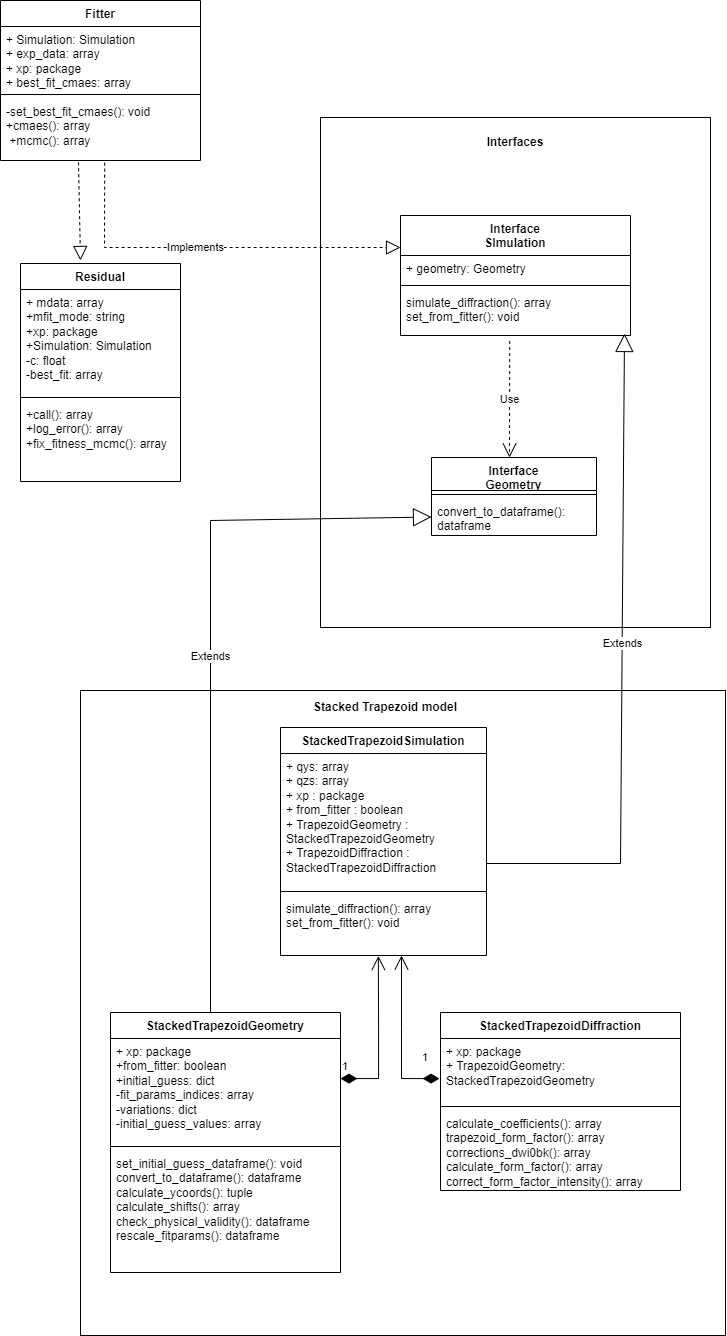
\includegraphics[width=0.7\textwidth]{images/cdsaxs_UML.png}
    \caption{UML diagram of the design for CD-SAXS simulation application. }
    \label{fig:UML}
\end{figure}

\FloatBarrier

\subsubsection*{\textbf{Simulation interface:}}

This is the base class for all simulation models. The functions and classes used in it should be implemented
in all simulation models.

\subsubsection*{\textbf{Geometry interface:}}

Like Simulation interface. This is the base class for all geometry models.


\subsubsection*{\textbf{Model:}}

In this UML diagram (Figure \ref{fig:UML}), we present the implementation of the stacked trapezoid model.
 Central to this model is the \textit{StackedTrapezoidSimulation} class, which is a composite class 
 integrating \textit{StackedTrapezoidGeometry} and \textit{StackedTrapezoidDiffraction} classes. The 
 \textit{StackedTrapezoidGeometry} class handles all geometrical calculations and stores the relevant 
 information, while the \textit{StackedTrapezoidDiffraction} class is responsible for all diffraction-related 
 calculations.

 \medskip

These classes work together to simulate the physics and generate data that can be compared with experimental
results. Throughout the project, additional models are being developed and they will be discussed later. The stacked 
trapezoid model serves as a prototype, illustrating how other models will be implemented. Each model will 
adhere to the base interfaces \textit{Simulation} and \textit{Geometry}.

\subsubsection{Relationships between components}

\medskip

This system is designed to simulate and analyze diffraction patterns using
 a modular approach. At its core, the system comprises several key components:
  the \textit{Fitter}, \textit{Residual}, and interfaces for \textit{Simulation}
   and \textit{Geometry}, along with specific model implementations like the
   \textit{StackedTrapezoidSimulation}. The \textit{Fitter} class orchestrates
the fitting process by using the \textit{cmaes} function to estimate the best-fit parameters and
 the \textit{mcmc} function to assess the uncertainty in the fit. It takes in a model and
  experimental data, utilising the \textit{Residual} class to compute the difference between
   the experimental data and the model's simulated data. The \textit{Residual} class leverages
    the model's \textit{simulate\_diffraction} function to generate the diffraction pattern,
     which it then compares with the experimental data.

\medskip

The model, meaning specific implementations of the interfaces, is designed to operate 
independently, allowing users to utilize a particular model
for simulations without needing to engage with the fitting component. This autonomous 
functionality ensures that users can easily perform simulations solely with the model of
 their choice. This design choice enhances flexibility and usability, as it decouples the simulation process from the fitting procedures, making it more accessible for users who may only need to run simulations.
The usefulness and implications of this design choice will be discussed shortly.


\subsubsection{Why this design?}
Let's first discuss the shortcomings of the previous design before explaining why the current design was chosen.

\subsubsection*{Previous design:}

The previous design adopted a monolithic approach, where the fitting and simulation components were tightly coupled. This meant that any changes to the fitting algorithm (e.g., adding a new optimization technique) would necessitate modifications to the simulation code as well. This interdependence made it difficult to introduce new functionalities or modify existing ones without potentially impacting other parts of the system.

\medskip

\begin{figure}[h]
    \centering
    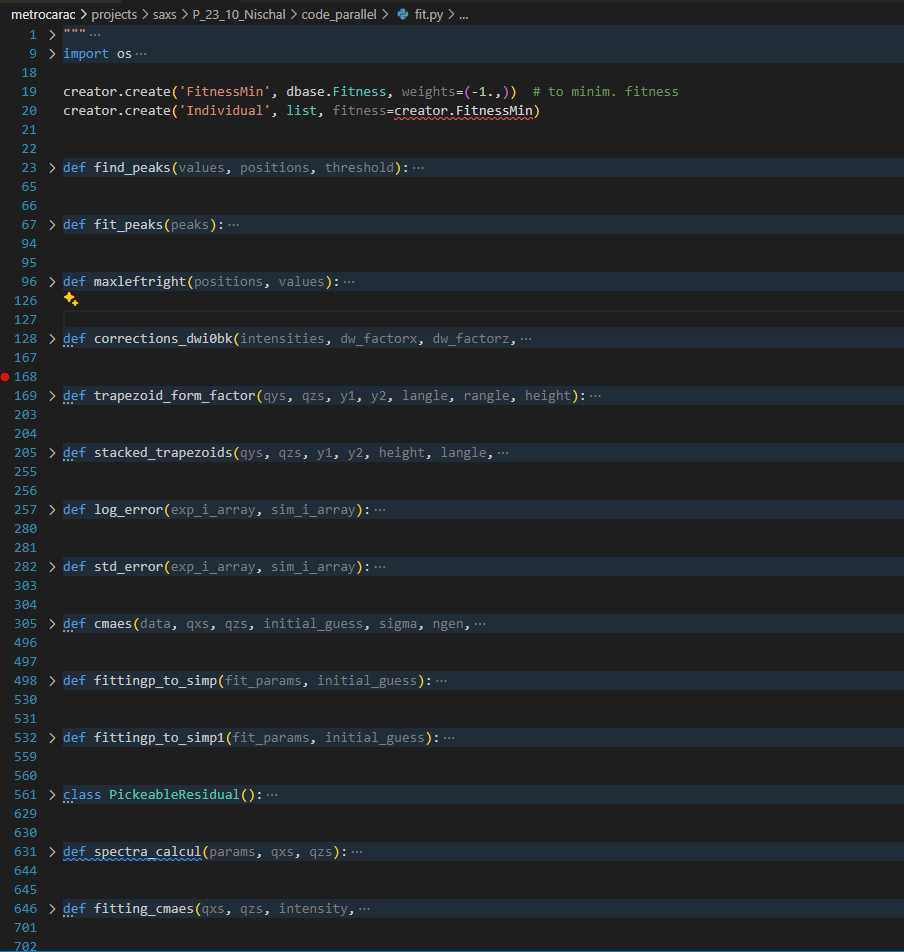
\includegraphics[width=0.5\textwidth]{images/monolithic.png}
    \caption{Monolithic design of the previous version. This script combined all the functions for the stacked trapezoid model
     in one file.}
    \label{fig:monolithic_design}
\end{figure}

Furthermore, individual models within the system implemented their own fitting and simulation functionalities. This resulted in a significant amount of code duplication, leading to inconsistencies between models. Moreover, adding new models required rewriting these functionalities from scratch, hindering the system's scalability. This approach proved inefficient for managing a growing number of models. These two limitations combined made it challenging to optimize or parallelize the code effectively. Since the fitting and simulation components were intertwined, it was difficult to isolate and optimize individual sections for improved performance.

\medskip

Similarly the codes for the different models each implemented their own fitting and simulation
components, leading to code duplication and inconsistencies across models. This design was not
scalable, as adding new models required rewriting the fitting and simulation components for each
model.

\subsubsection*{Current design:}

The current design improves upon the previous version by decoupling the fitting and 
simulation components, resulting in a modular structure. The \textit{Simulation} interface serves
 as the connecter between fitting and simulation, standardizing the process of fitting 
 any model.

\medskip

Also, by enabling simulation models to be developed independently of the fitting component, 
new models can be introduced without modifying the existing codebase. Developers can 
focus on developing new models without concerning themselves with the fitting process. 
This design choice significantly enhances the system's flexibility and scalability.

\medskip

The decoupling of components also facilitates optimization and 
parallelization by allowing developers to focus on specific areas of improvement without
 cross-component interference. For example, the simulation component can be optimized to
  run faster and more efficiently through advanced numerical methods and parallel 
  computing techniques. This is particularly beneficial for handling large datasets or complex simulations that demand significant computational resources. By isolating the simulation component, developers can experiment with and implement various optimization strategies, ensuring that the component runs as efficiently as possible.

\subsection{Simulation Models}

During my project there were three main models that are planned to be integrated with the application. 
In this section I will discuss the idea behind each model and how they were or are in the process of being implemented in the code.
For each model, We will also shortly discuss the lithography technique and/or fault that it is designed to simulate.

\subsubsection{Stacked Trapezoid Model}





\subsection{Implementation of MCMC}
\subsection{Optimisation and parrellelisation}
\subsection{On the fly uncertainity estimation}